\documentclass[a4paper]{article}

\usepackage[utf8]{inputenc}
\usepackage[english]{babel}
\usepackage{fancyhdr,graphicx}
\usepackage[colorlinks=true,linkcolor=black,urlcolor=blue,bookmarksopen=true]{hyperref}

\newcommand{\materia}{[75.41] Taller de Programación I}
\newcommand{\trabajo}{Manual de usuario}
\newcommand{\trabajoheader}{Ejercicio final }
\newcommand{\cuatri}{1c2019}
\newcommand{\cuatrimestre}{Primer cuatrimestre de 2019}
\newcommand{\grupo}{Grupo 3}

\newcommand{\autores}{
	Camila Bojman,
	Cecilia Hortas,
	Nicolas Vazquez}

\hypersetup{
	pdftitle={\trabajo},
	pdfsubject={\materia},
	pdfauthor={\autores},
}

\pagestyle{fancy}
\fancyhf{}
\fancyhead[L]{\materia}
\fancyhead[R]{\trabajoheader - \trabajo}
\renewcommand{\headrulewidth}{0.4pt}
\fancyfoot[C]{\thepage}
\renewcommand{\footrulewidth}{0.4pt}

\begin{document}
	\pagenumbering{gobble}
	\pagenumbering{roman}
	\pagenumbering{arabic}
	\setcounter{page}{1}
	
	\begin{titlepage}
		\hfill
\includegraphics[width=6cm]{fiuba.jpeg}
		\begin{center}
			\vfill
			\Huge \textbf{\trabajo}
			\vskip2cm
			\Large \materia\\
			\cuatrimestre
			\vfill
			\grupo
			\begin{itemize}
				\item Camila Bojman 101055 camiboj@gmail.com
				\item Cecilia Hortas 100687 ceci.hortas@gmail.com
				\item Nicolas Vazquez 100338 vazquez.nicolas.daniel@gmail.com
			\end{itemize}
			\vskip1cm
		\end{center}
	\end{titlepage}

\section{Instalación}

\subsection{Requerimientos de software}

\subsection{Requerimientos de hardware}

\subsection{Proceso de instalación}

\section{Configuración}

La configuración del juego se realiza por medio de un archivo de formato \texttt{YAML} que se encuentra localizado en la carpeta \texttt{config} dentro de la carpeta \texttt{server} del repositorio. Hay ciertos parámetros comunes que pueden variarse, pero se recomienda mantenerlos dentro del mismo rango para obtener el juego que fue testeado numerosas veces por sus creadores.

\section{Forma de uso del juego}
El juego es de tipo \textit{cooperativo}, lo que implica que para finalizar la partida todos deben alcanzar el objetivo reconocido como victoria. En este caso particular, \textbf{todos} los jugadores deben llegar a la llamada \textit{cake} que se trata de una torta localizada en algún lugar del escenario. Para ello deberán sortear con distintos obstáculos, en los cuales podrían morir. En el caso en que un jugador muera, esto no genera ninguna diferencia en la condición de victoria, incluso a veces puede ser necesario por ejemplo si todo el grupo llegó a la torta y un solo jugador quedó varado en el camino. En esta implementación del juego portal hay 3 causas de muerte:
\begin{enumerate}
	\item Si una bola de energia choca a Chell desde cualquier posición
	\item Si una roca cae encima de Chell
	\item Si Chell toca ácido accidentalmente
\end{enumerate}

A continuación se enumeran los distintos movimientos habilitados por las teclas del teclado:
\begin{itemize}
	\item \textbf{a} para moverse a la izquierda.
	\item \textbf{d} para moverse a la derecha.
	\item \textbf{w} para saltar.
	\item \textbf{g} para agarrar una roca. Un dato a tener en cuenta es que en caso de existir más de una roca en el escenario, se designará la que se encuentre a menor distancia del jugador en cuestión.
	\item \textbf{f} para dejar la roca en algún lugar en particular. Esto puede ser útil para abrir una compuerta (colocar una roca sobre un botón) o asesinar a otro jugador (tirándole una roca encima).
	\item \textbf{t} para lanzar una roca hacia arriba. Esta funcionalidad fue agregada para poder transportar una roca a través de un portal.
	\item \textbf{clic derecho} para lanzar un disparo con intenciones de colocar un portal de color naranja. 
	\item \textbf{clic izquierdo} para lanzar un disparo con intenciones de colocar un portal de color azul. 
	\item \textbf{r} para borrar los portales creados por el mismo jugador.
	\item \textbf{p} para colocar un \textit{pintool} en cualquier lugar de la pantalla. Para eso debe moverse el mouse hasta la posición determinada y luego presionar la tecla susodicha.
	\item \textbf{o} para eliminar el pintool puesto por el mismo jugador.
\end{itemize}

Ahora para poder localizar la torta es necesario moverse por el escenario, en el cual el usuario podría encontrarse con alguna dificultad u objeto desconocido. Se enumeran una serie de preceptos a tener en cuenta a la hora de jugar el juego:
\begin{itemize}
	\item Tener en cuenta que se puede crear un portal de color azul y un portal de color naranja por jugador y que sólo pueden crearse sobre los bloques de metal. Así mismo, la creación de un portal naranja elimina cualquier otro portal naranja creado \textbf{por el mismo jugador}. Obviamente no interfiere con portales creados por otros jugadores. Si el disparo no choca con algún bloque de metal, simplemente no hace nada.
	
	\item El ácido es letal. Como fue mencionado previamente, Chell al tocarlo se muere inmediatamente.
	
	\item Existen emisores y receptores de bolas de energía. El emisor lanza bolas de energía cada cierto período de tiempo, las cuales asesinan a Chell en el acto si se topan con ella. Hay 4 tipos de emisores: el que lanza bolas de energía para la izquierda, derecha, arriba o abajo. La idea de estas bolas de energía, además de representar un peligro para Chell, es llegar a un receptor de energía y activarlo. Esta activación es útil porque puede llegar a ser requerida para abrir una puerta cerrada del escenario. Por último existen nuevamente los mismos tipos de receptores de energía.
	
	\item Una puerta puede estar cerrada. Para abrirla se necesita cumplir con una cierta condición lógica que puede implicar el uso de los operadores lógicos \texttt{and}, \texttt{or} y \texttt{not} y se realiza sobre los botones y receptores de energía. Por ejemplo, puede haber una puerta que para ser abierta deba tener activado un receptor de energía y un botón. Para ello debería esperarse que una bola de energía sea emitida por un emisor hacia dicho receptor y colocar una roca u otro jugador sobre un botón.
	
	\item Se debe tener en cuenta que las bolas de energía, si bien tienen una dirección fija al ser lanzadas por el emisor, pueden toparse con un portal y teletransportarse además de cambiar su dirección al toparse con un bloque con dirección diagonal o rebotar sobre un bloque de metal. Sobre un bloque de roca no sucederá nada debido a que la asesina en el acto.

	\item Solamente se pueden colocar portales sobre bloques de metal. Intentar hacerlo sobre cualquier otro objeto es en vano.
	
	\item La roca se desintegra completamente al toparse con una barra de energía. Igualmente no representa en un peligro en sí para Chell.
	
	\item Si una roca y una bola de energía colisionan, ambas mueren en el acto.
	
	\item Pueden teletransportarse rocas por los portales de manera de acceder a otros lugares del escenario, donde puede ser necesario activar un botón. Para hacerlo, como se mencionó previamente se recomienda lanzar la roca hacia arriba o abandonarla si el portal está por debajo.
	
	\item Existe el objeto \texttt{pintool} para armonizar el trabajo en grupo y llegar al pastel. Este elemento se utiliza para que un jugador indique a otro que estaría bueno que cree un portal ahí para cumplir el objetivo del nivel. Queda a completa responsabilidad del usuario ser inteligente con el mismo y colocarlo de la manera más estratégica posible. Así mismo, mueren después de un determinado tiempo y no pueden crearse más de uno por jugador, por lo que la creación de un segundo pin tool en el escenario por parte del mismo jugador elimina inmediatamente el anterior.
	
	\item Se pueden resetear tanto los portales como los pintools de manera de utilizar otra combinación más estratégica.
\end{itemize}

\subsection{Ejemplo de uso}

A continuación se muestra un ejemplo de uso del juego. Este se trata de un nivel confeccionado por el \texttt{Editor} que refleja las funcionalidades básicas del juego. Se explicará cómo usar el mismo luego.

En un primer lugar se muestra la forma en la que se ve una piedra cuando Chell la agarra. La idea es levantarla del piso y que su movimiento esté acoplado al de Chell. Es decir, si Chell se mueve para la derecha o izquierda, la roca sigue su movimiento. Chell no puede saltar con una roca pero sí puede lanzarla hacia arriba o dejarla en el piso.

\begin{figure}[!h]
	\makebox[\textwidth][c]{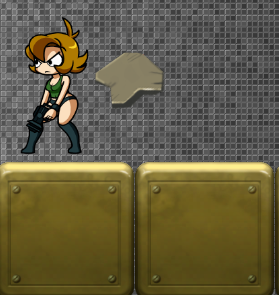
\includegraphics[width=0.5\textwidth]{Holding_rock.png}}
	\caption{Chell agarra roca}
	\label{fig:diagrama1}
\end{figure}

La idea de llevar rocas y utilizarlas es principalmente para colocarlas sobre botones y así abrir las puertas que impiden que Chell llegue a un lugar específico. Observando el siguiente ejemplo, se ve que la puerta está cerrada y que debería activarse al menos un botón para abrir la puerta. Puede pasar en el desarrollo del juego que el jugador deba tantear la condición lógica ya que no se mostrará explícitamente la misma en pantalla para motivar la estrategia. En este caso puntual deben activarse ambos botones para poder abrirla, como puede observarse en la \textit{Figura 3}. Vale la pena recordar que la activación del botón se realiza tanto con el peso de una piedra como de otro jugador.

\begin{figure}[!h]
	\makebox[\textwidth][c]{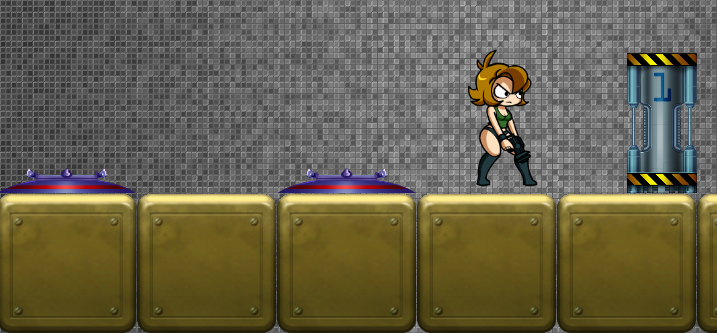
\includegraphics[width=0.5\textwidth]{Door_closed.png}}
	\caption{Puerta cerrada}
	\label{fig:diagrama2}
\end{figure}


\begin{figure}[!h]
	\makebox[\textwidth][c]{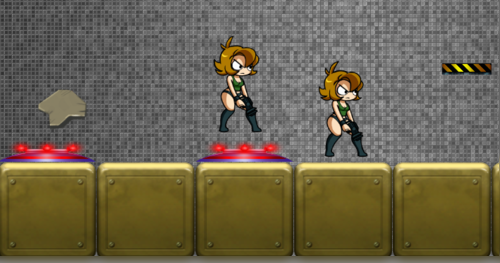
\includegraphics[width=0.5\textwidth]{Door_open.png}}
	\caption{Puerta abierta}
	\label{fig:diagrama3}
\end{figure}

Ahora sí, al inicio de este nivel se presenta la siguiente situación: la puerta está cerrada y el botón está más arriba de lo que Chell puede lanzar una piedra (además de que sería un movimiento en vertical difícil de alcanzar). Además Chell no puede saltar con la piedra y tampoco puede activarla con su propio peso porque hay solo un jugador.

\begin{figure}[!h]
	\makebox[\textwidth][c]{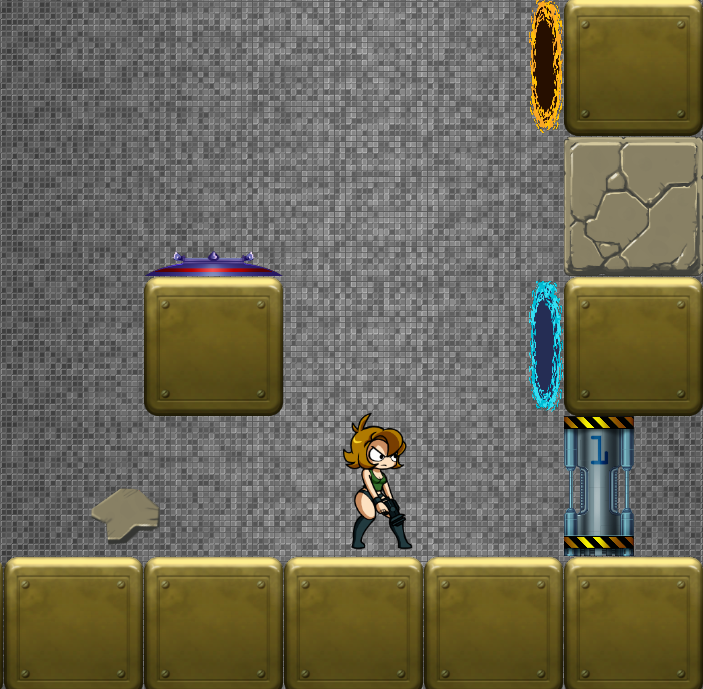
\includegraphics[width=0.5\textwidth]{Strategy.png}}
	\caption{Primer desafío}
	\label{fig:diagrama4}
\end{figure}

Una posible solución (y probablemente no la única) es hacerle caso al nombre del juego y crear un portal para lanzar la piedra y que llegue al botón y así abrir la puerta. Hay que recordar que los bloques de roca no permiten la creación de portales por lo que la única alternativa es crear los portales en los bloques de metal. Por supuesto los portales podrían ubicarse de otra forma, invertirlos (uno azul arriba y uno naranja abajo), poner alguno en el piso y otro más arriba, cualquier opción en la cual el usuario se sienta más cómodo. Hay que recordar que si la piedra toca la cabeza de Chell se muere en el instante por lo que se recomienda tomar la opción que resulte más segura.

\begin{figure}[!h]
	\makebox[\textwidth][c]{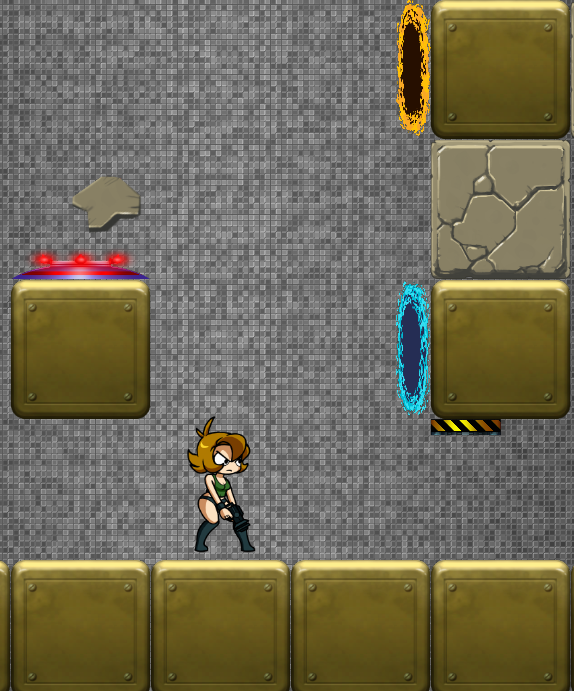
\includegraphics[width=0.5\textwidth]{Strategy_open.png}}
	\caption{Primer desafío superado}
	\label{fig:diagrama5}
\end{figure}

Ahora se presenta un nuevo desafío: el ácido es letal y hay que llegar a la \textit{cake} para ganar el juego.

\begin{figure}[!h]
	\makebox[\textwidth][c]{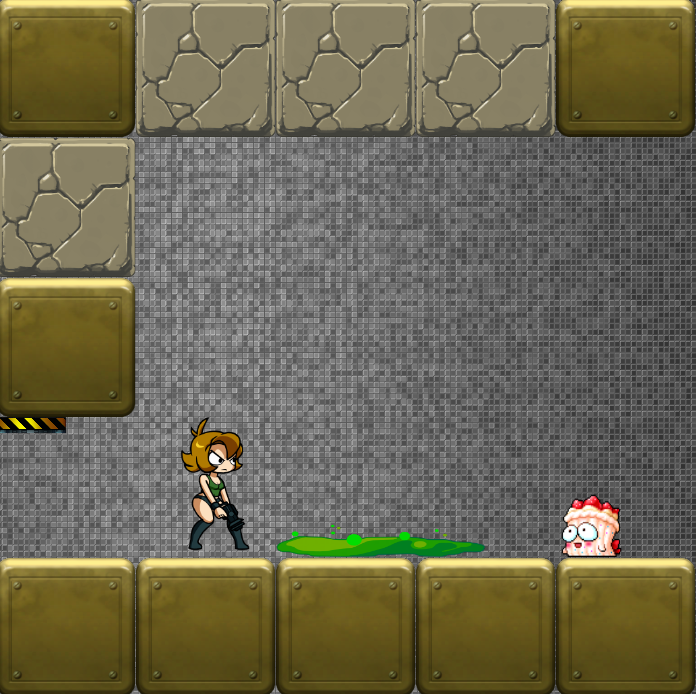
\includegraphics[width=0.5\textwidth]{Reaching_the_cake.png}}
	\caption{Segundo desafío}
	\label{fig:diagrama6}
\end{figure}

Una posible solución sería saltar ese ácido, pero eso podría resultar arriesgado. Por lo tanto, se recurre nuevamente a los famosos portales para llegar al objetivo. No es casualidad que el nivel esté diseñado de manera tal que los únicos dos bloques donde se puede realizar portales sean los que resulten más beneficiosos al jugador. Recordar que la creación de dos nuevos portales borran automáticamente los anteriores.


\begin{figure}[!h]
	\makebox[\textwidth][c]{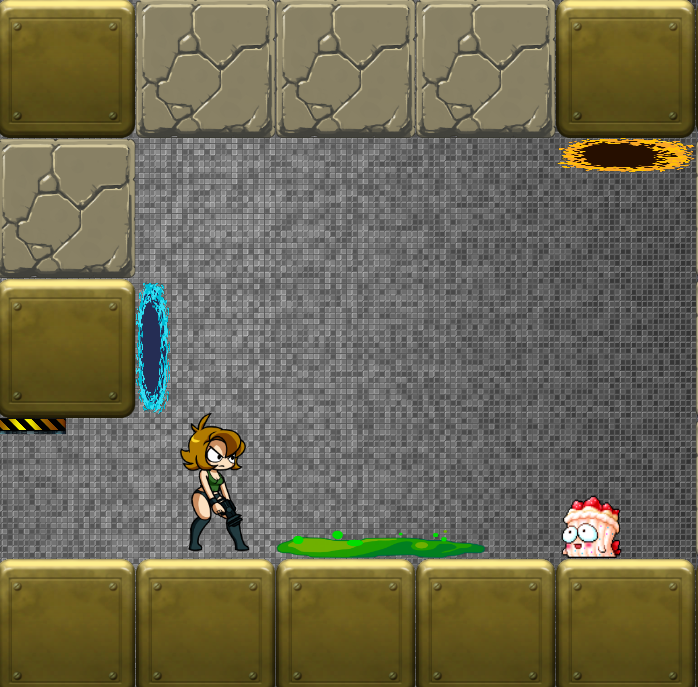
\includegraphics[width=0.5\textwidth]{Cake_reached.png}}
	\caption{Segundo desafío superado}
	\label{fig:diagrama7}
\end{figure}

\subsection{Muestra de objetos}

Ahora se presentan otros elementos del juego para que el usuario se familiarice con los mismos. 

En un primer lugar, se muestra una bola de energía, transmitida por un emisor y una barra de energía horizontal colocada por encima de un bloque de metal. Como fue mencionado previamente la barra de energía permite el traspaso de bolas de energía y de Chell, pero no así de las rocas y los disparos. En este ejemplo Chell debería esperar el momento en el que la bola de energía no puede tocarla ya que es letal para ella.

\begin{figure}[!h]
	\makebox[\textwidth][c]{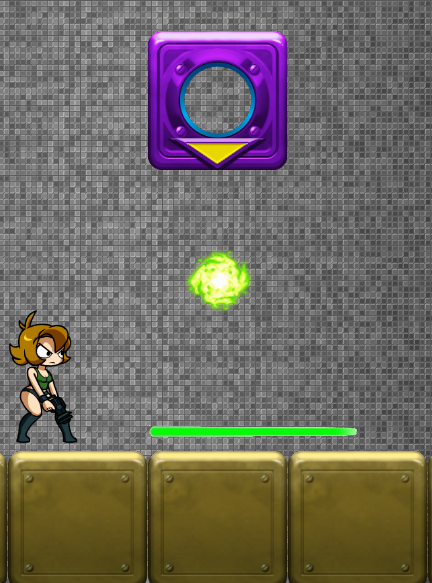
\includegraphics[width=0.5\textwidth]{Energyball_eb.png}}
	\caption{Bola de energía y barra de energía}
	\label{fig:diagrama8}
\end{figure}

Otra función que cumplen las bolas de energía es activar los llamados receptores, utilizados para la lógica de compuertas. Esta activación consiste en que la bola de energía colisione con la "boca" del receptor. Una vez activado, queda activado por siempre y \textit{puede} permitir abrir una puerta. Hay casos en los que por la disposición de los emisores y receptores, los receptores serán activados por estar en la trayectoria de la bola. Podría suceder que no sea así y que para activarlo se deba crear un portal que teletransporte la bola de energía y cambie su trayectoria.

En la \textit{Figura 9} se observa un emisor que emite bolas de energía hacia arriba y un receptor que las recibe desde abajo. Se muestra la diferencia entre un receptor desactivado (primer caso) y un receptor activado (segundo caso).

\begin{figure}[!h]
	\makebox[\textwidth][c]{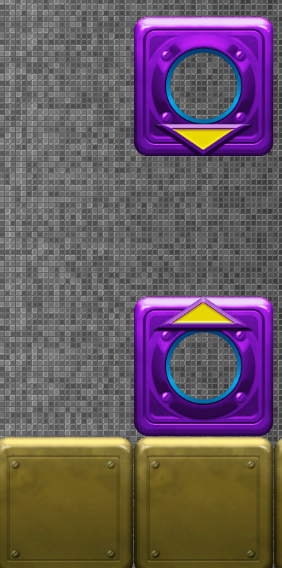
\includegraphics[width=0.25\textwidth]{er_off.png}}
	\caption{Receptor desactivado}
	\label{fig:diagrama9}
\end{figure}

\begin{figure}[!h]
	\makebox[\textwidth][c]{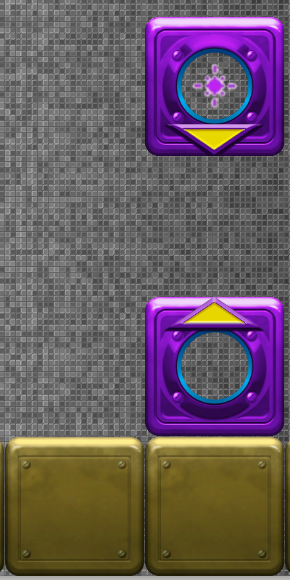
\includegraphics[width=0.25\textwidth]{er_on.png}}
	\caption{Receptor activado}
	\label{fig:diagrama10}
\end{figure}

Cabe recordar que las bolas de energía rebotan contra un bloque de metal u otro emisor, pero mueren contra un bloque de roca. Se observa en la \textit{Figura 10} que la bola de energía rebota contra el bloque de metal.

\begin{figure}[!h]
	\makebox[\textwidth][c]{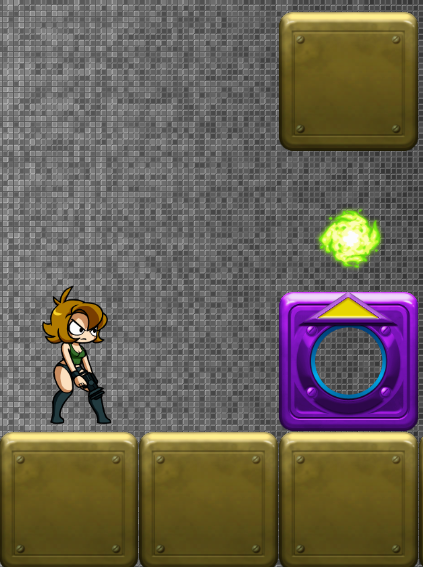
\includegraphics[width=0.5\textwidth]{eb_bounce.png}}
	\caption{Bola de energía rebota en bloque de metal}
	\label{fig:diagrama11}
\end{figure}

Por último un caso especial es el de los bloques en diagonal. Chell resbala por los mismos si camina por encima y las bolas de energía al rebotar contra ellas cambian su dirección. Es importante tener en cuenta esto porque Chell puede estar posicionada en una dirección que no está en la trayectoria de la bola designada por el emisor e ignorar el hecho que puede chocarla en cualquier momento por dicho desvío.

\begin{figure}[!h]
	\makebox[\textwidth][c]{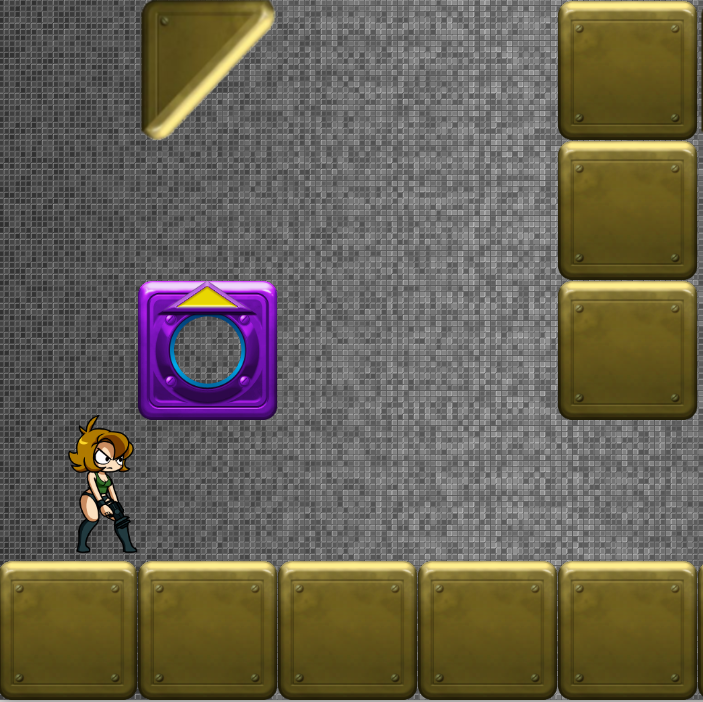
\includegraphics[width=0.5\textwidth]{diagonal_1.png}}
	\caption{Bola de energía cambia direccion en bloque de metal diagonal}
	\label{fig:diagrama12}
\end{figure}

Se observa en las siguientes figuras que la bola de energia inicialmente presenta una trayectoria horizontal y luego sigue una trayectoria paralela a la normal de la hipotenusa del bloque en diagonal.

\begin{figure}[!h]
	\makebox[\textwidth][c]{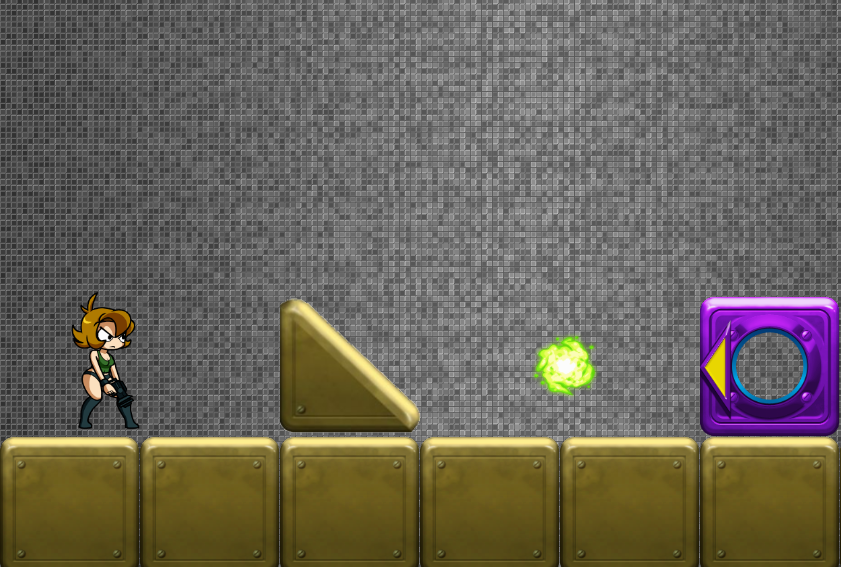
\includegraphics[width=0.5\textwidth]{diagonal_2.png}}
	\caption{Bola de energía cambia direccion en bloque de metal diagonal}
	\label{fig:diagrama13}
\end{figure}

\begin{figure}[!h]
	\makebox[\textwidth][c]{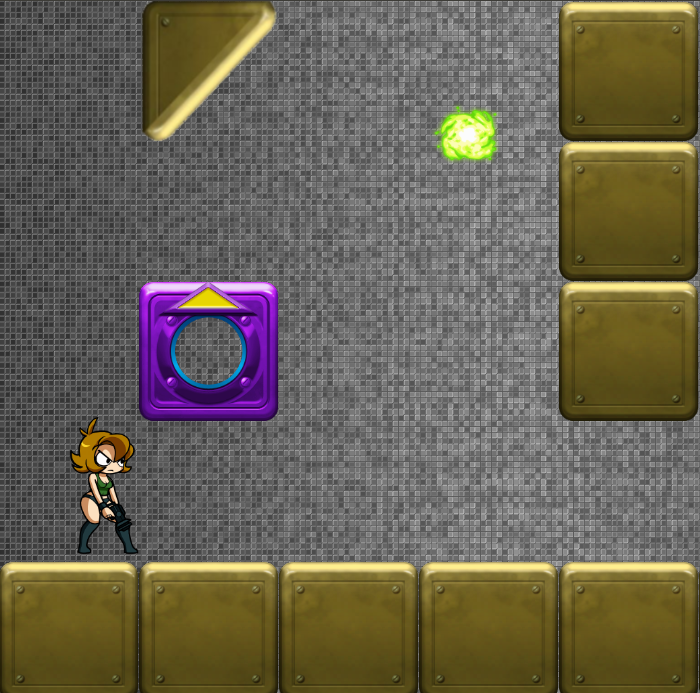
\includegraphics[width=0.5\textwidth]{diagonal_3.png}}
	\caption{Bola de energía cambia direccion en bloque de metal diagonal}
	\label{fig:diagrama14}
\end{figure}

\begin{figure}[!h]
	\makebox[\textwidth][c]{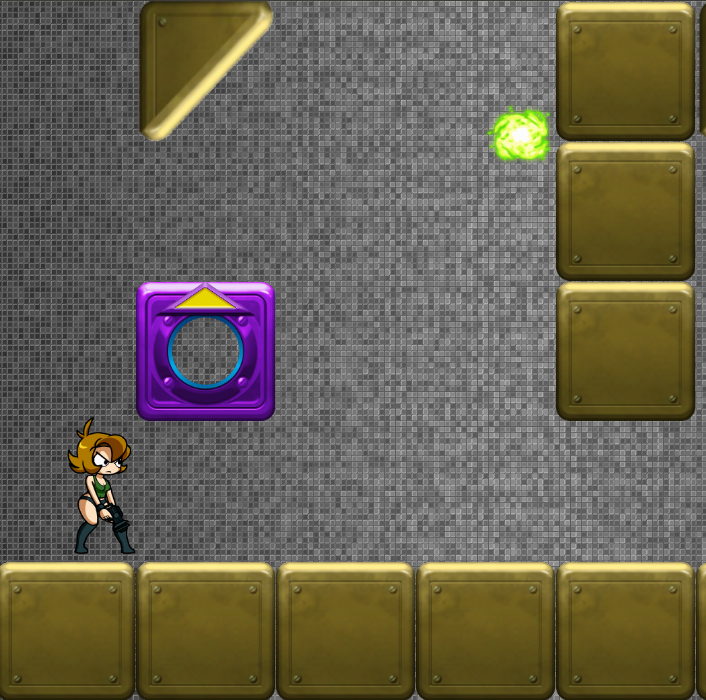
\includegraphics[width=0.5\textwidth]{diagonal_4.png}}
	\caption{Bola de energía cambia direccion en bloque de metal diagonal}
	\label{fig:diagrama15}
\end{figure}

\newpage 

\section{Forma de uso del editor}
El editor se utiliza para crear o editar los niveles de juego. Pueden disponerse los elementos en la posición que el usuario desee y guardarlo todo en un archivo que luego será seleccionado al iniciar el juego.

Al iniciar el editor se observará la siguiente pantalla:

\begin{figure}[!h]
	\makebox[\textwidth][c]{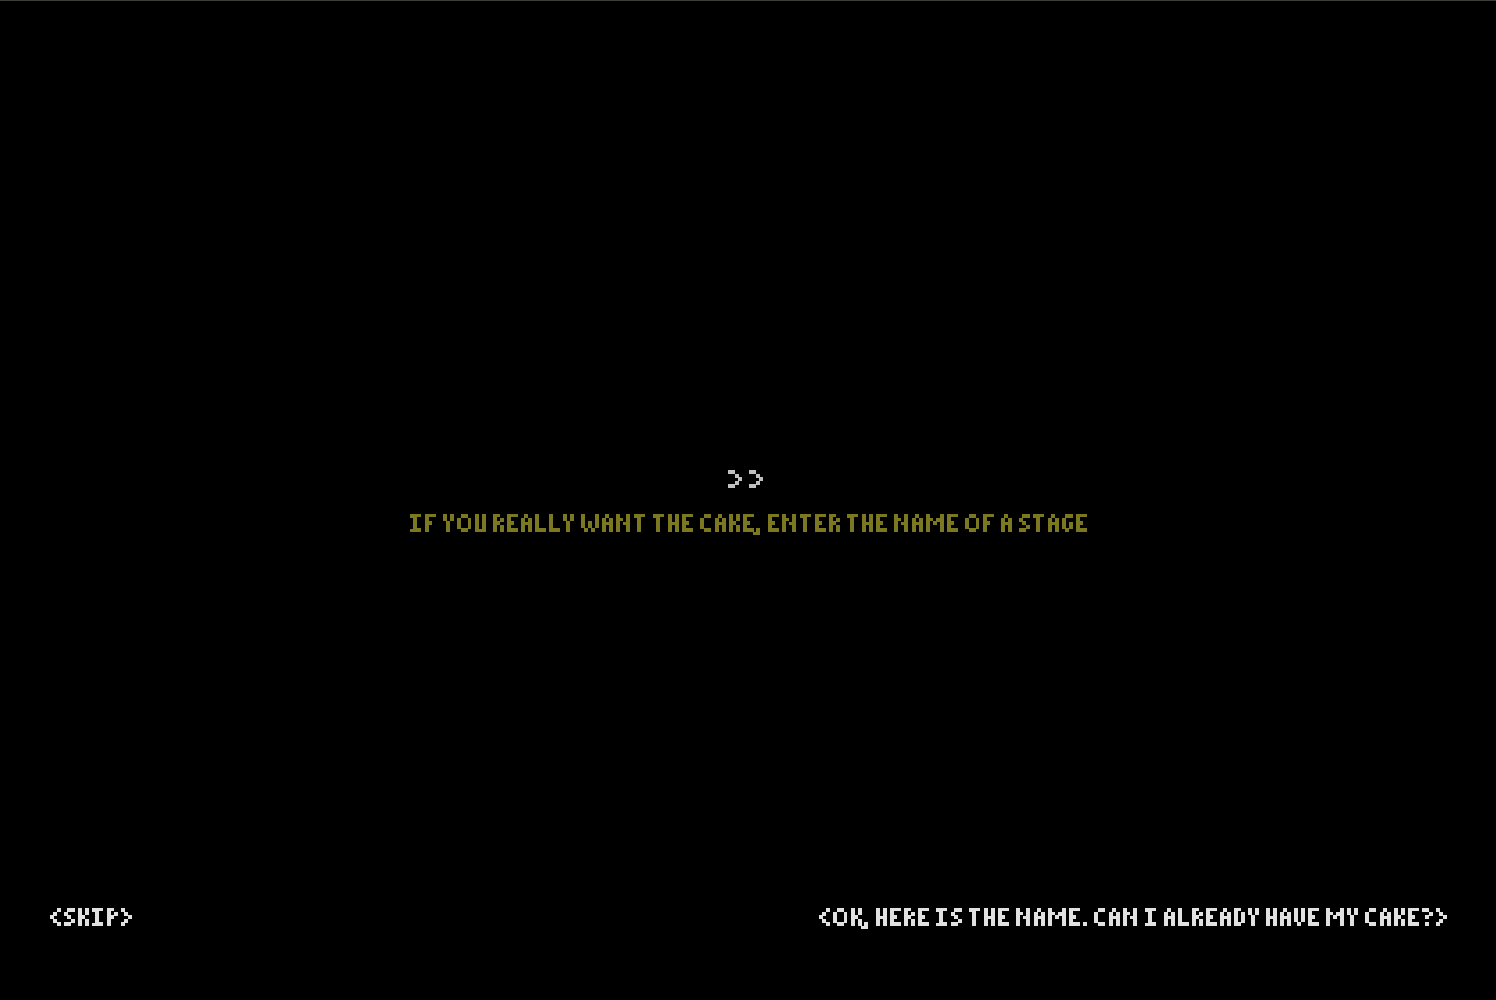
\includegraphics[width=1\textwidth]{editor_initial.png}}
	\caption{Pantalla de inicio del editor}
	\label{fig:diagrama16}
\end{figure}

Aquí puede escribirse el nombre del nivel que se desea editar y hacer clic en \texttt{OK, HERE IS THE NAME, CAN I ALREADY HAVE MY CAKE?} o decidir iniciar un nuevo nivel y hacer clic en \texttt{<SKIP>}. 

Una vez elegido esto, aparece la pantalla dispuesta en la \textit{Figura 17} que es el editor en sí mismo. Se puede observar que aparecen todos los elementos descritos en la sección anterior. La forma de uso consiste en arrastrar los elementos al escenario de la manera que se desee. Si se desea cambiar de lugar un elemento simplemente se arrastra hacia el lugar deseado y si se desea eliminar se arrastra afuera de la pantalla. 

Por otro lado, para respetar ciertas leyes físicas, se impide la colocación de los objetos que obedecen la ley de la gravedad sobre la nada para evitar que caigan al iniciar el juego. Estos son el botón, Chell, la compuerta, las rocas, la \textit{cake} y el ácido. Esto quiere decir que sólo pueden colocarse sobre los bloques de metal, de piedra y los emisores y receptores. Si se desea hacer lo contrario, se imprime el siguiente mensaje de error en la terminal: \texttt{Couldn't add the tile: That's not a valid place for an object with physics laws!}.

Se muestra en la \textit{Figura 18} un ejemplo de nivel editado para mostrar a los objetos con ley de gravedad bien dispuestos y la posición libre del resto de los objetos.

\begin{figure}[!h]
	\makebox[\textwidth][c]{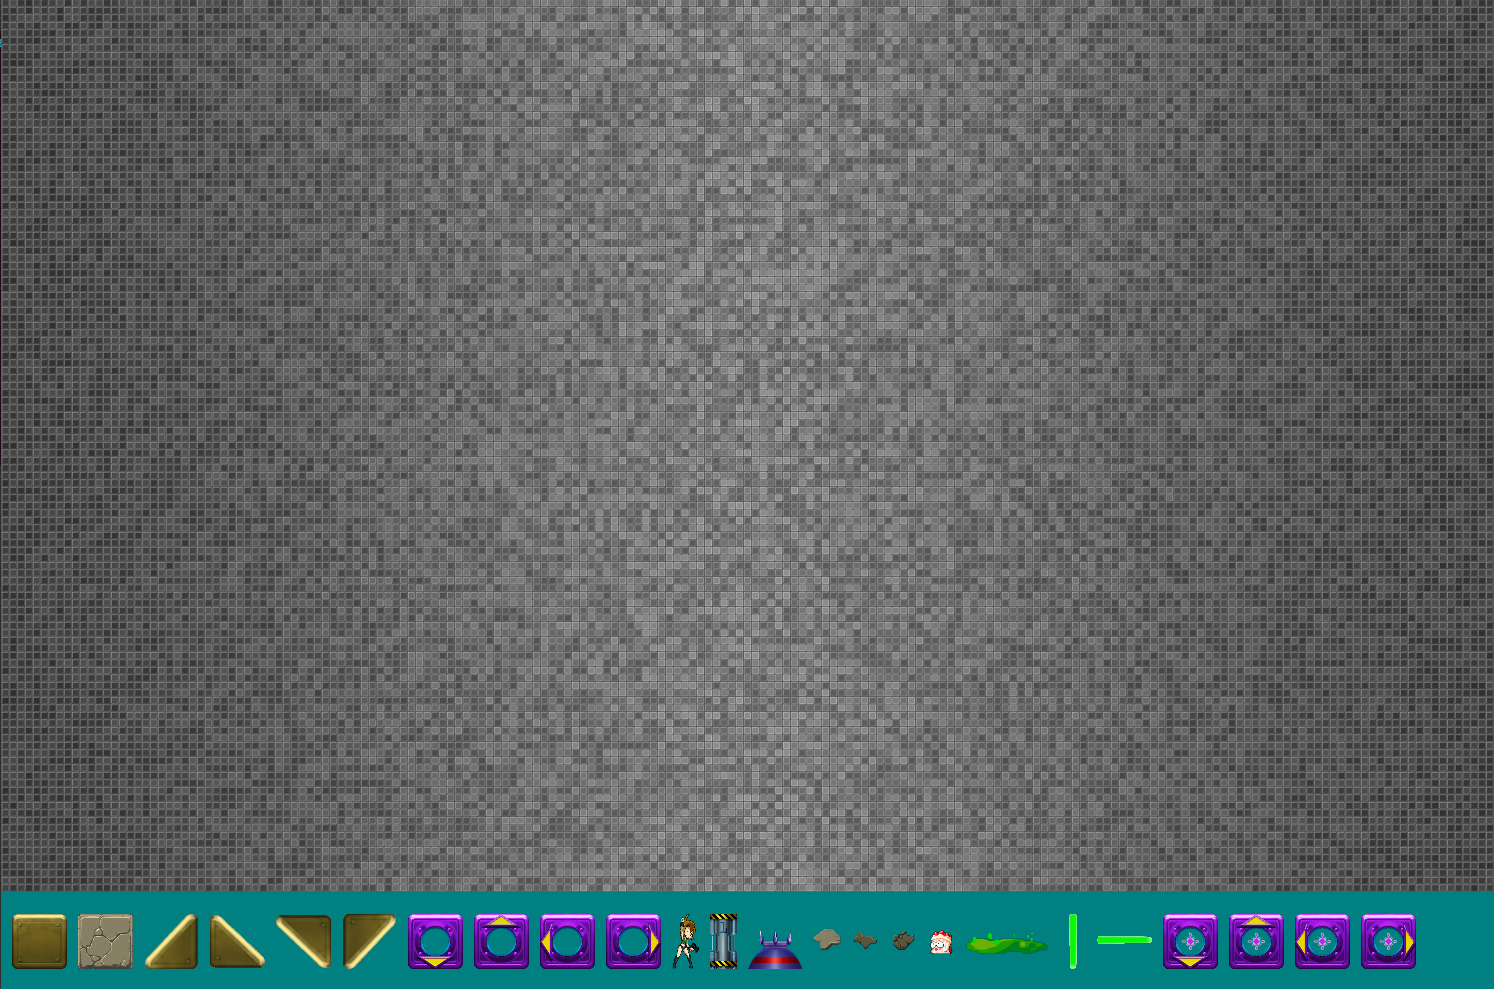
\includegraphics[width=1\textwidth]{editor.png}}
	\caption{Editor}
	\label{fig:diagrama17}
\end{figure}

\begin{figure}[!h]
	\makebox[\textwidth][c]{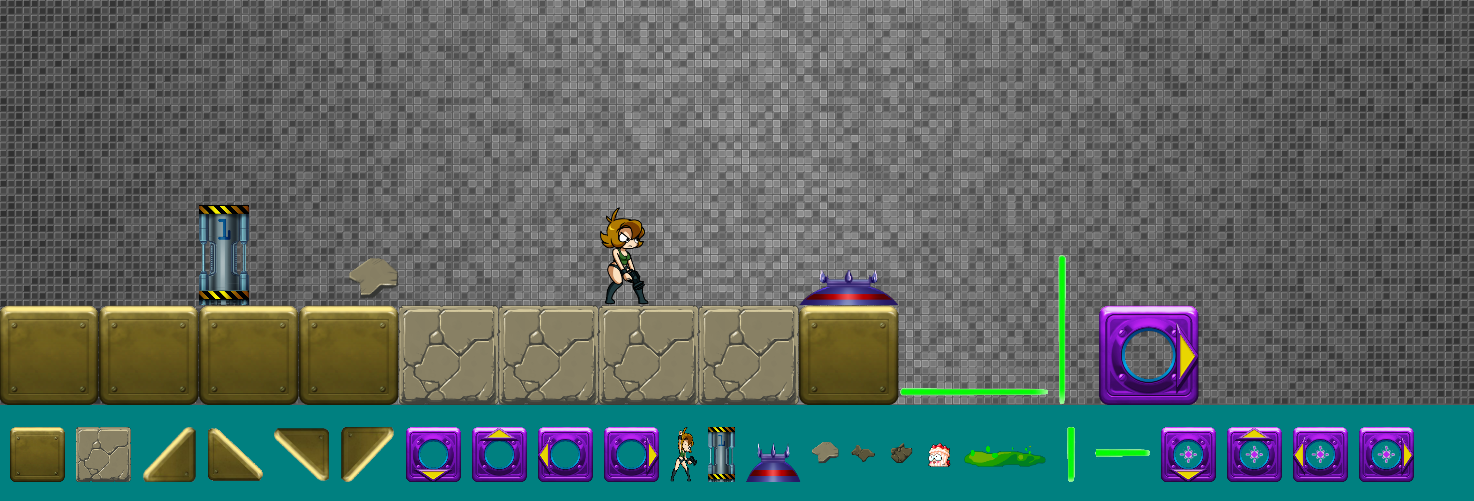
\includegraphics[width=1\textwidth]{example.png}}
	\caption{Ejemplo de edición}
	\label{fig:diagrama18}
\end{figure}

\newpage

Otra característica del editor es la posibilidad de hacer el escenario \textit{infinito} y moverlo para seleccionar los diversos objetos y posicionarlos en el lugar deseado. Esto se hace con las \textbf{flechas izquierda y derecha} del teclado y las teclas \textbf{a} y \textbf{d}. Un ejemplo de cómo se ve el escenario luego de correr el escenario hacia la derecha y abajo se observa en la \textit{Figura 19}

\begin{figure}[!h]
	\makebox[\textwidth][c]{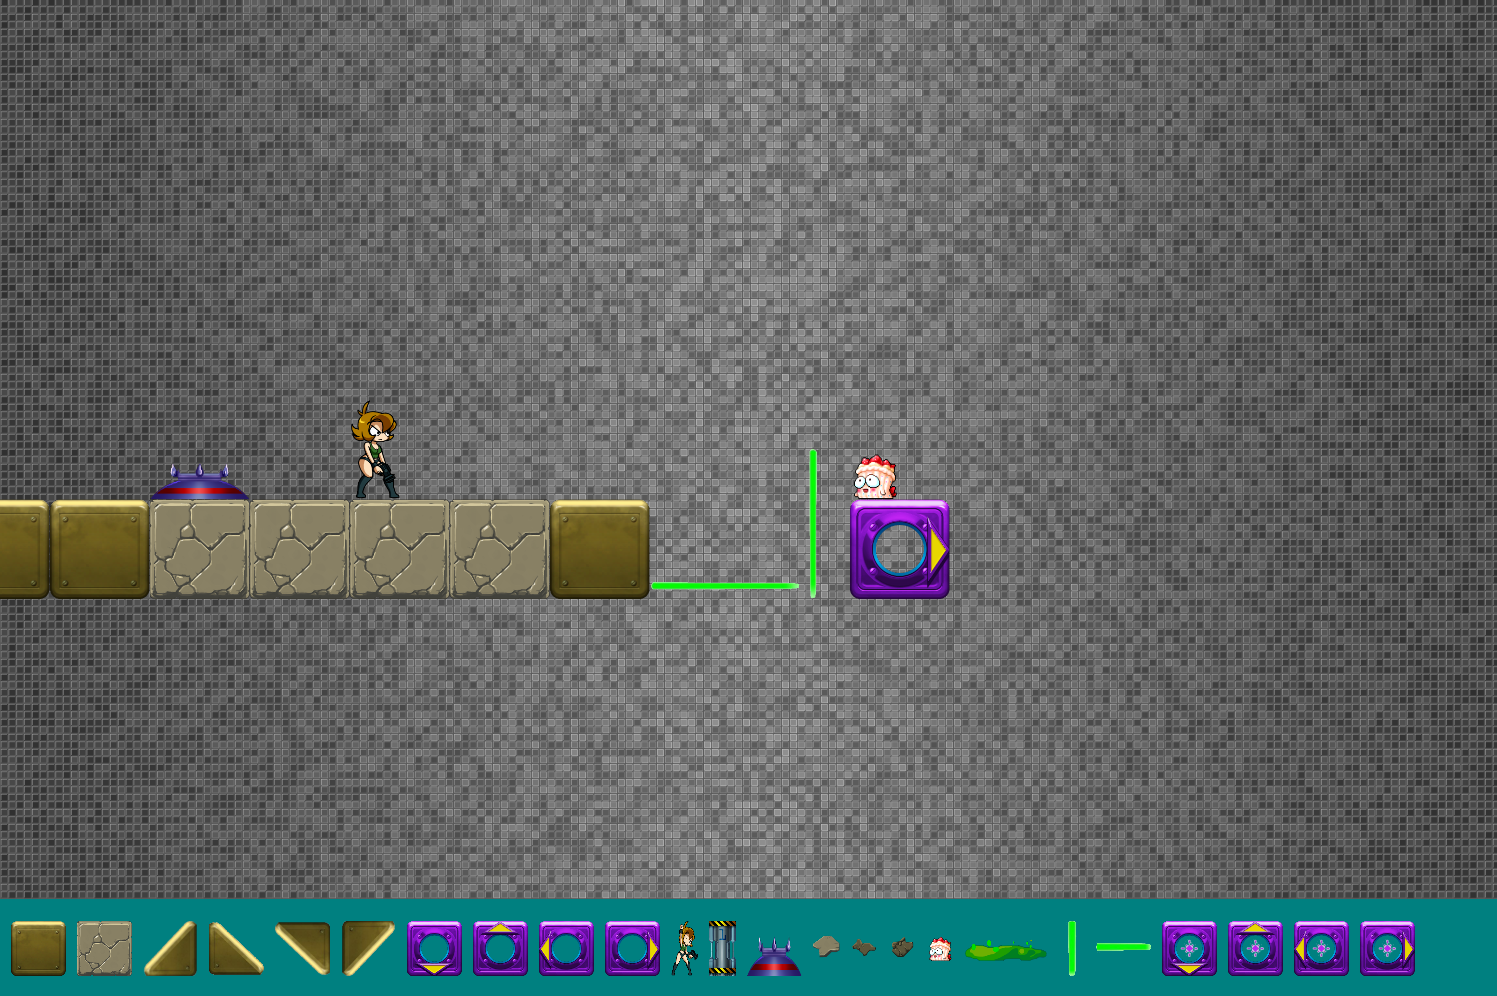
\includegraphics[width=1\textwidth]{infinit.png}}
	\caption{Editor infinito}
	\label{fig:diagrama19}
\end{figure}

\newpage

Un tema aparte es la lógica de compuertas y botones y receptores. Para designar un nombre a un botón o receptor basta con hacer \textbf{doble cliz izquierdo} sobre el mismo y escribir el nombre. Se puede observar en la primera figura el caso de nombrar a un botón y en la segunda el de nombrar a un receptor. Para designar una condición a una compuerta se hace \textbf{clic derecho} sobre la misma y se escribe la condición, luego apretando \textbf{enter} o haciendo \textbf{clic} en el \texttt{OK} que figura en pantalla.

En el caso que no se asigne un nombre a un botón o receptor, ese botón simplemente no se tiene en cuenta para la lógica de compuertas y así mismo si no se designa una condición a una compuerta, la misma pertenece abierta por default.

\begin{figure}[!h]
	\makebox[\textwidth][c]{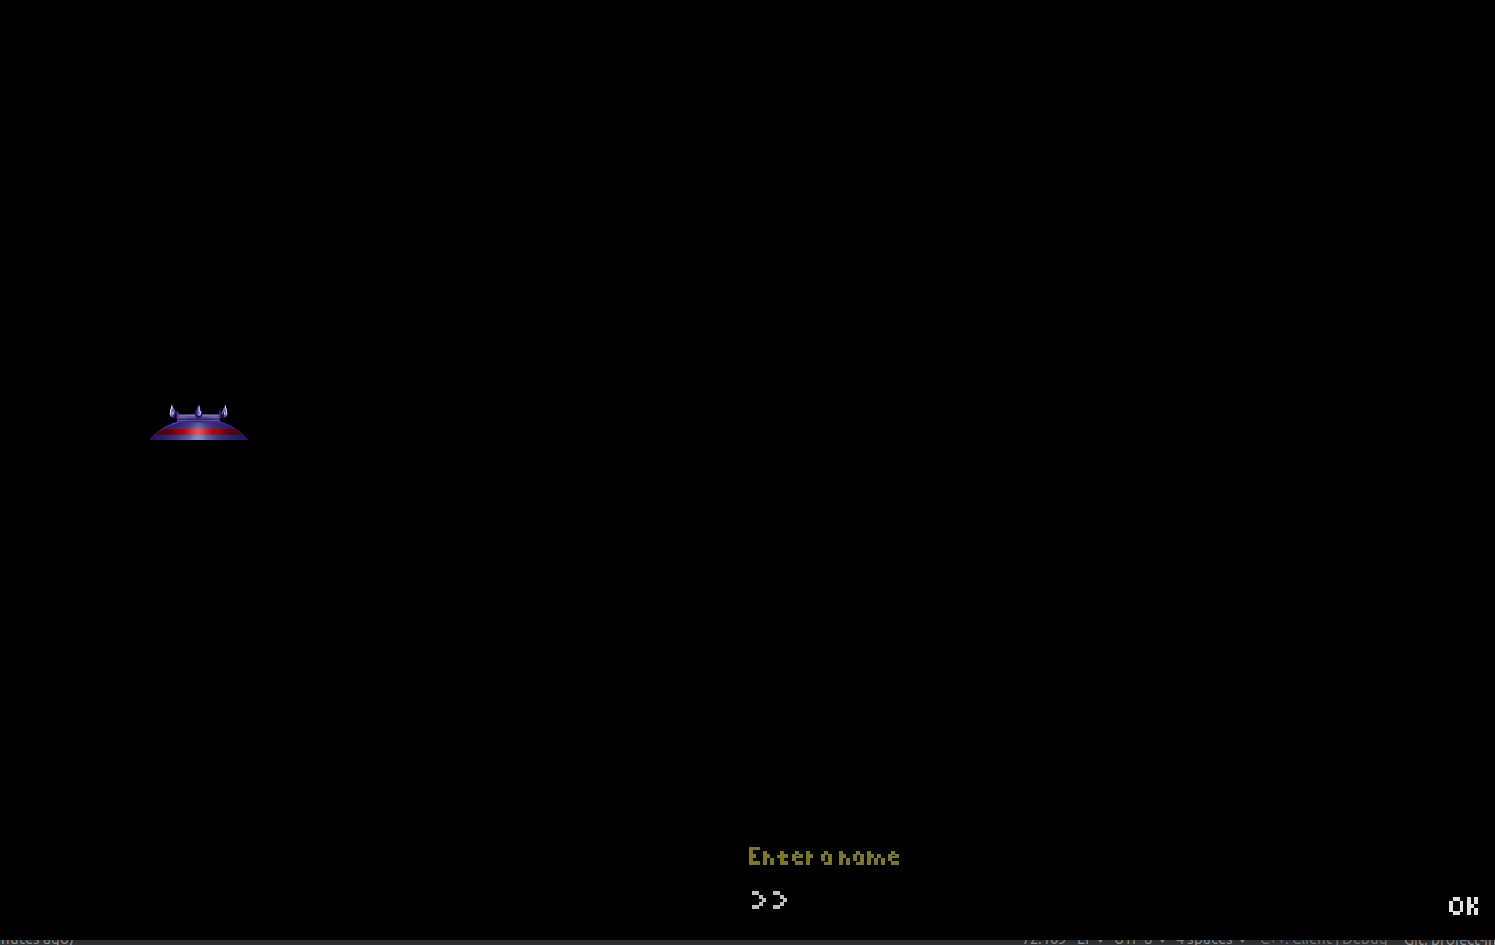
\includegraphics[width=0.75\textwidth]{button.png}}
	\caption{Designar nombre a un botón}
	\label{fig:diagrama20}
\end{figure}

\begin{figure}[!h]
	\makebox[\textwidth][c]{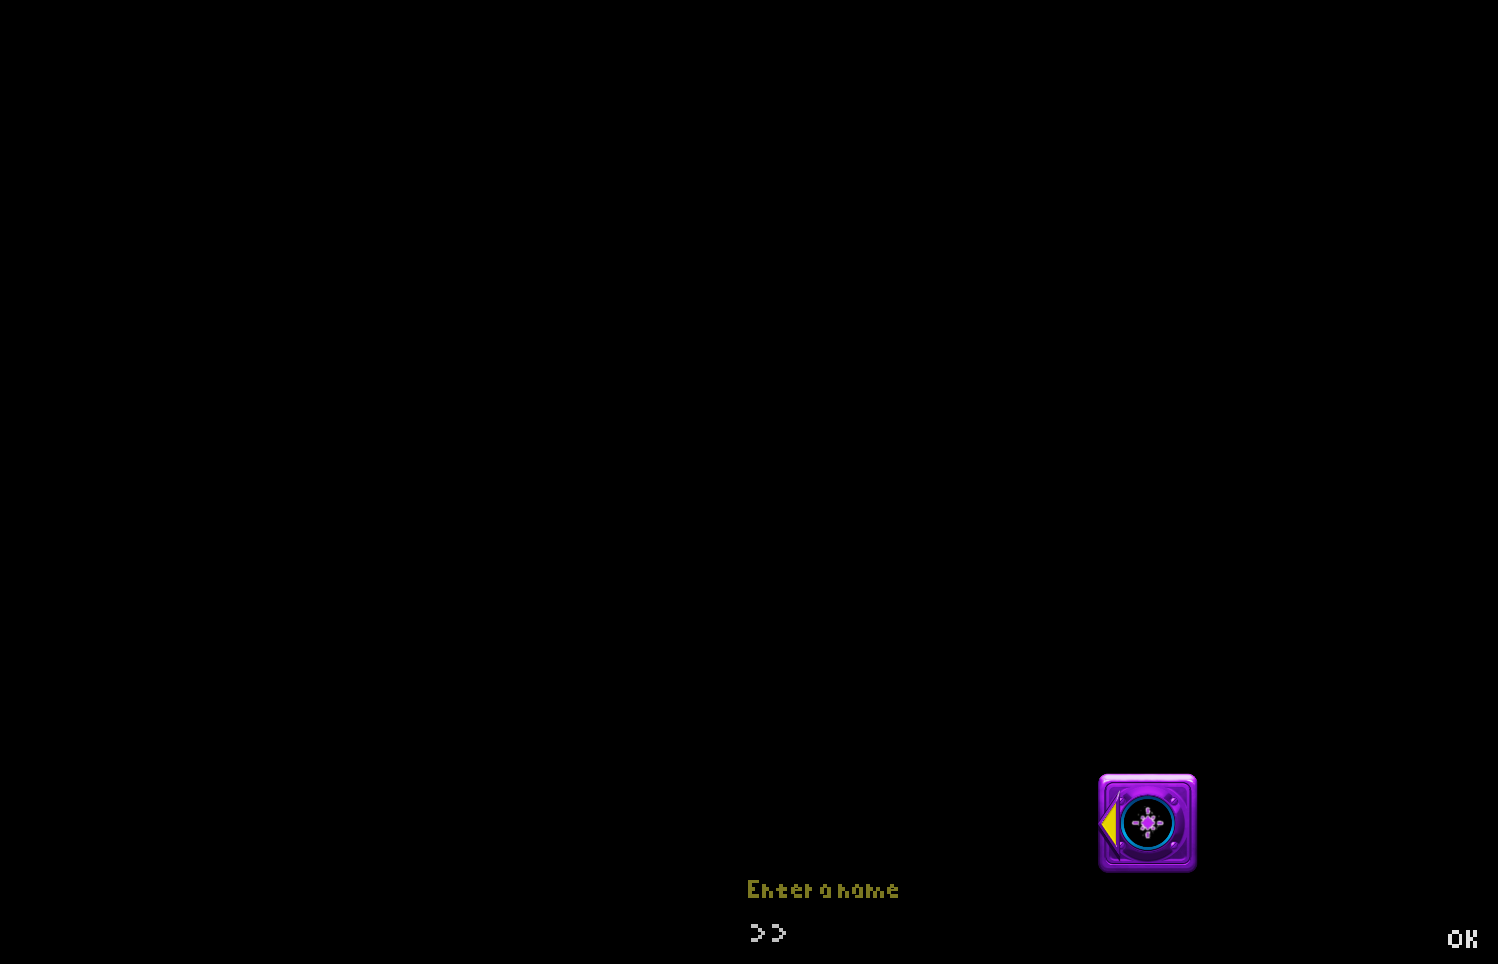
\includegraphics[width=0.75\textwidth]{receptor.png}}
	\caption{Designar nombre a un receptor}
	\label{fig:diagrama21}
\end{figure}

\begin{figure}[!h]
	\makebox[\textwidth][c]{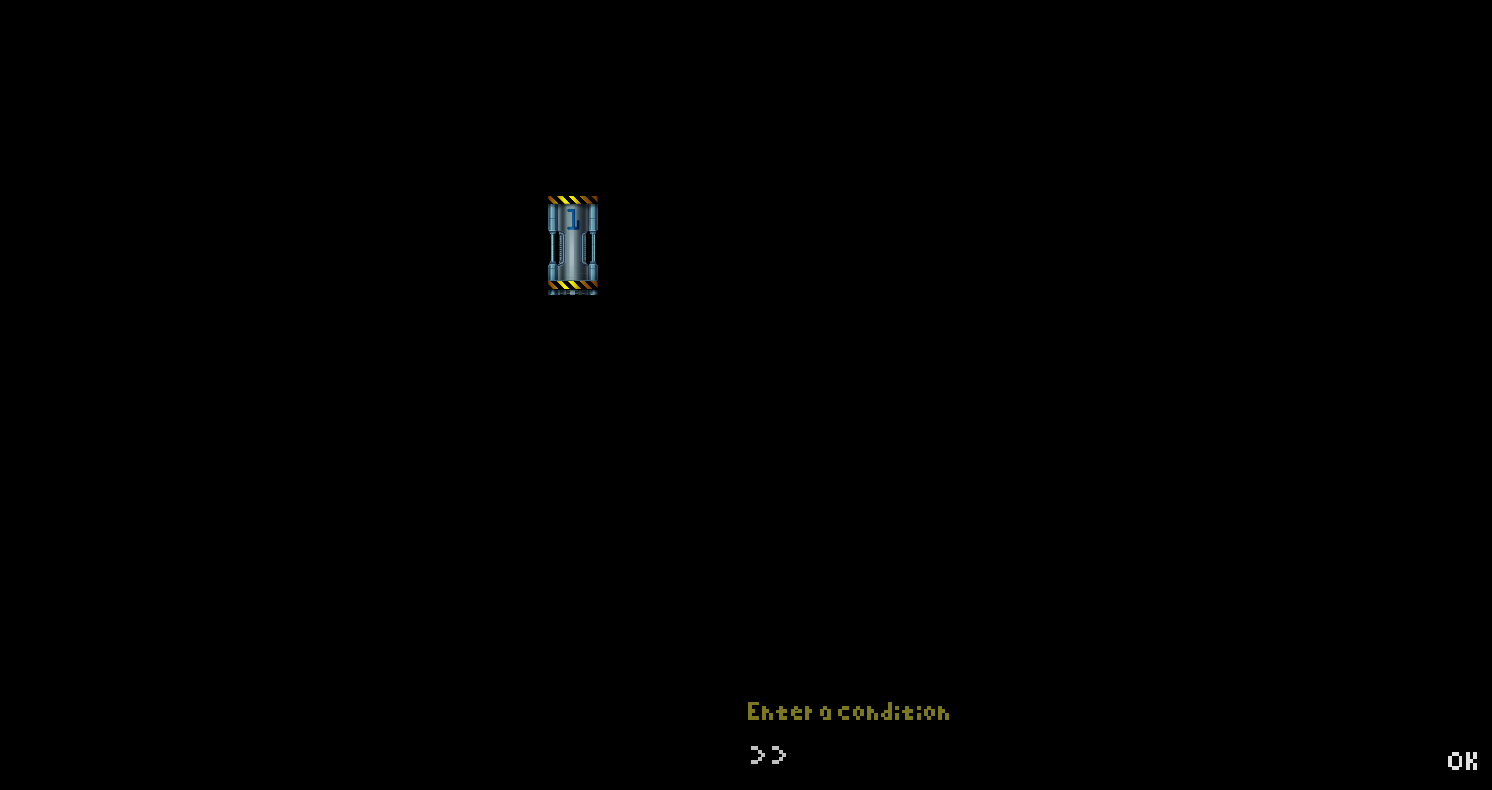
\includegraphics[width=0.75\textwidth]{condition.png}}
	\caption{Designar una condición a una compuerta}
	\label{fig:diagrama22}
\end{figure}

\newpage

Una vez finalizada la edición, el mismo se guarda haciendo \textbf{CTRL+S} y se escribe el nombre del nivel que se desea utilizar.

\begin{figure}[!h]
	\makebox[\textwidth][c]{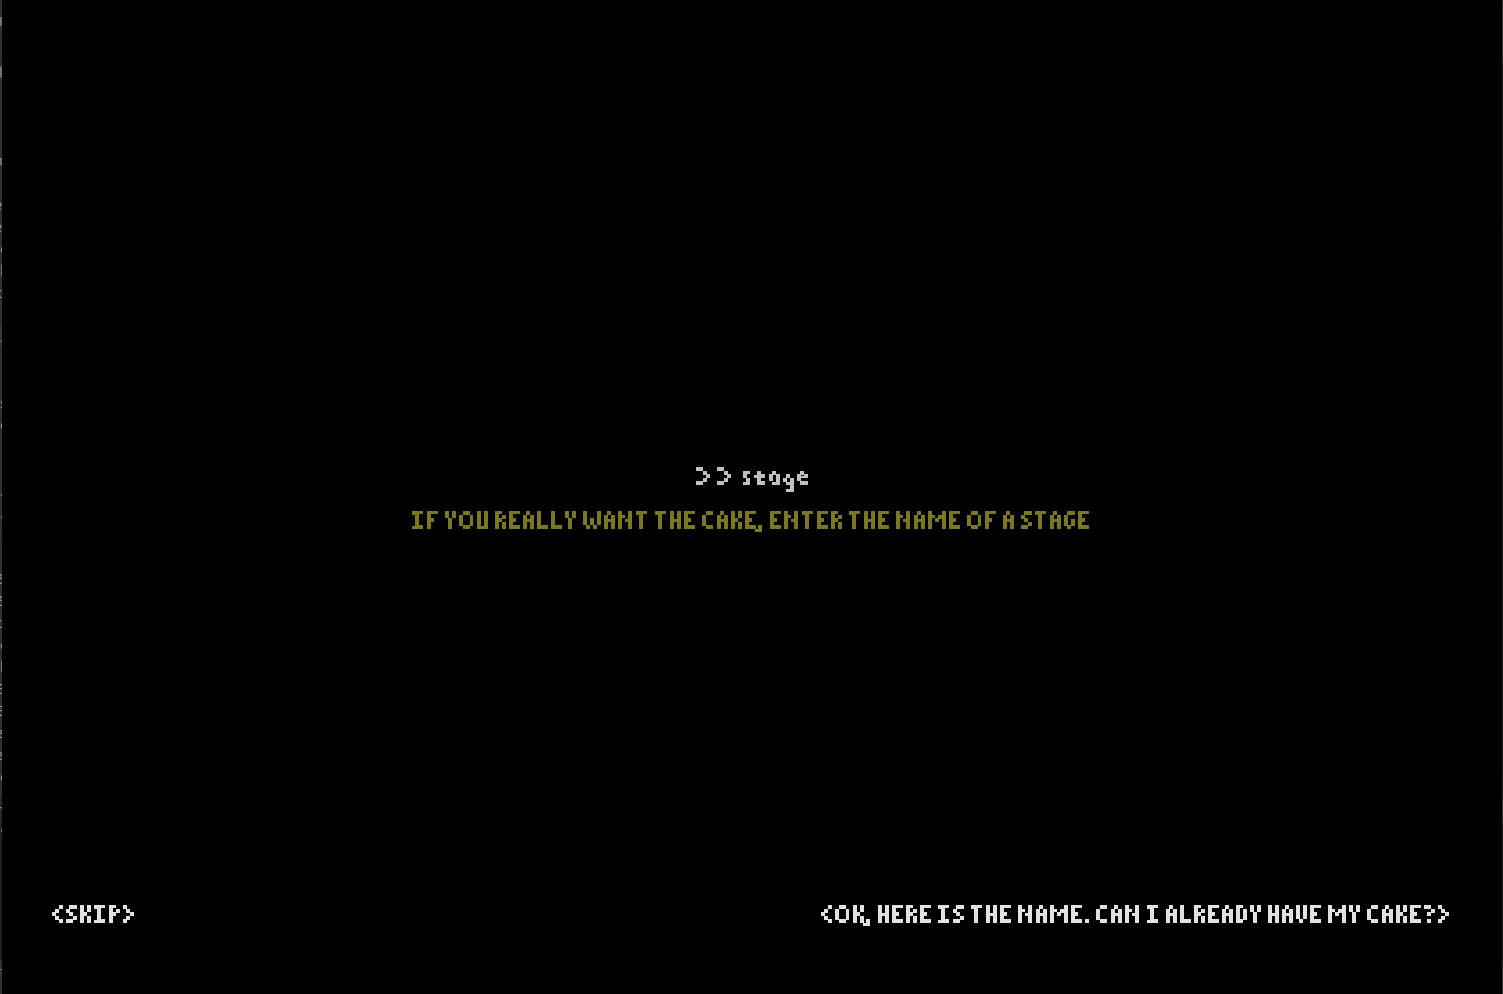
\includegraphics[width=1\textwidth]{saving_editor.png}}
	\caption{Guardar un nivel en el editor}
	\label{fig:diagrama23}
\end{figure}

Luego en el juego se puede seleccionar un nivel en el momento de creación del juego. Se muestra una serie de niveles a elegir y el usuario escribe el que haya seleccionado. Los últimos pasos para la creación de una partida es elegir un nombre para el juego y un ID. La cantidad de jugadores está predefinida por el editor, por lo que si se edita un nivel con 3 jugadores deberán conectarse 3 clientes para comenzar el juego. La unión a una partida se configura seleccionando alguno de los juegos disponibles y eligiendo un ID (distinto al de los jugadores en juego). El juego se desarrolla hasta que se gana (todos llegan a la \textit{cake}) o se pierde (todos mueren), mostrando un mensaje por pantalla que indica el resultado y finaliza la ejecución.

\end{document}